\chapter{Data Selection}
\label{cha:data_selection}
The selected dataset onto which a classification model shall be learned is provided by Kaggle \footnote{2017 Kaggle Inc}. It is named \textit{The movies Dataset}\footnote{Link to the dataset: \hyperref[https://www.kaggle.com/rounakbanik/the-movies-dataset]{https://www.kaggle.com/rounakbanik/the-movies-dataset}} and contains metadata on approximately 45,000 movies in its raw format. It is provided and updated by Rounik Banik. The complete dataset consits out of several files in the \textit{.csv} format containing specific info about movie casts, and external score. For the outcome of this project the central file, used for further preprocessing is named \textit{movies-metadata.csv}. This csv-file holds 24 columns in total, which can be expected in the graphic below.\\\\
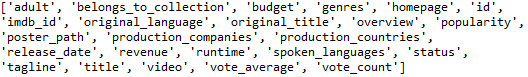
\includegraphics[width=\textwidth]{images/Raw_dataset_headers.png}
Untertitel bla bla

\section{Structure and size of data}

\section{Basic data exploration}

\begin{itemize}
	\item In slides named: "structure and size of data"
	\item min. 1 Page
	\item Selection: 
	\begin{itemize}
		\item What data is available?
		\item What do I know about the provenance of the data?
		\item What do I know about the quality of the data?
		\item Wrong values, lot of null values
	\end{itemize}
	\item Exploration
	\begin{itemize}
		\item Get an initial understanding of the data
		\item Calculate basic summarization statistics
		\item Visualize the data
		\item Identify data problems such as outliers, missing values, duplicate records
		\item problem with number scales, data formats, truth of contents
	\end{itemize}
\end{itemize}

Main issue quality of data. Further explained in preprocessing...
